\documentclass{article}

\usepackage{tikz}
\usetikzlibrary{automata, positioning, arrows}

\begin{document}

\begin{figure}[ht]
\begin{center}
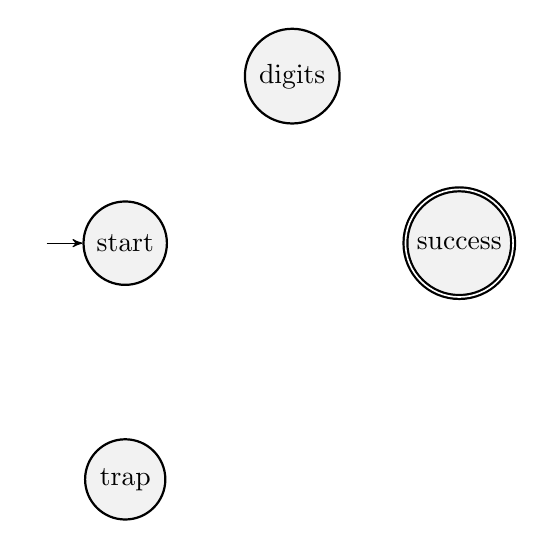
\begin{tikzpicture}
[->,
 >=stealth',
 node distance=3cm,
 every state/.style={thick, fill=gray!10,
 initial text=$ $}
]
\node[state] (digits) {digits};
\node[state, initial, below left of=digits] (start) {start};
\node[state, below of=start] (trap) {trap};
\node[state, below right of=digits, accepting] (success) {success};

% \draw (<source node>) edge[<edge options>] node{<edge label>} (<dest node>);
\end{tikzpicture}
\end{center}
\end{figure}

\end{document}